%% =====================================================================================
%% main.tex  AAMAS 2027 submission, built on the OFFICIAL template (aamas.cls).
%%
%% Template files are copied verbatim from aamas_2027_template.zip: aamas.cls,
%% ACM-Reference-Format.bst, by.pdf, by.eps. Do not edit them, and do not change any
%% layout parameter (CFP: "Please do not modify the style files or any of the layout
%% parameters"). The copyright block below is the template's own, unchanged.
%%
%% BUILD (from the repository root):
%%   python paper/AAMAS/analysis/selfplay.py
%%   python paper/AAMAS/analysis/overview.py      (reads num_selfplay.tex, so after selfplay)
%%   python paper/AAMAS/analysis/probes.py
%%   python paper/AAMAS/analysis/scripted.py
%%   python paper/AAMAS/analysis/mixed.py
%%   python paper/AAMAS/analysis/advantage.py
%%   python paper/AAMAS/analysis/selection.py
%%   cd paper/AAMAS && latexmk -pdf main.tex
%% Supplementary material (a separate PDF; AAMAS allows no appendix in this file):
%%   python paper/AAMAS/supplement/make_prompts.py
%%   cd paper/AAMAS/supplement && latexmk -pdf supplement.tex
%% Model names: every reader-facing name carries its family (Claude Haiku, Gemini
%% Flash-Lite, GPT Luna, Qwen, Grok); analysis/crsd_data.py DISPLAY is the one source.
%%
%% Every number in the prose is a macro written by one of those scripts. Do not type a
%% measured number into a section; add a macro to the script instead. Rule constants
%% (6 players, 10 rounds, 40 units, target 120, actions 0/2/4) are definitions and may be
%% typed.
%% =====================================================================================
\documentclass[sigconf,anonymous]{aamas}

\usepackage{balance}
\usepackage{booktabs}
\usepackage{array}
\usepackage{graphicx}
\usepackage{amsmath}

\makeatletter
\@ifundefined{proposition}{\theoremstyle{plain}\newtheorem{proposition}{Proposition}}{}
\makeatother

%%% AAMAS-2027 copyright block (do not change!)
\makeatletter
\gdef\@copyrightpermission{
  \begin{minipage}{0.2\columnwidth}
   \href{https://creativecommons.org/licenses/by/4.0/}{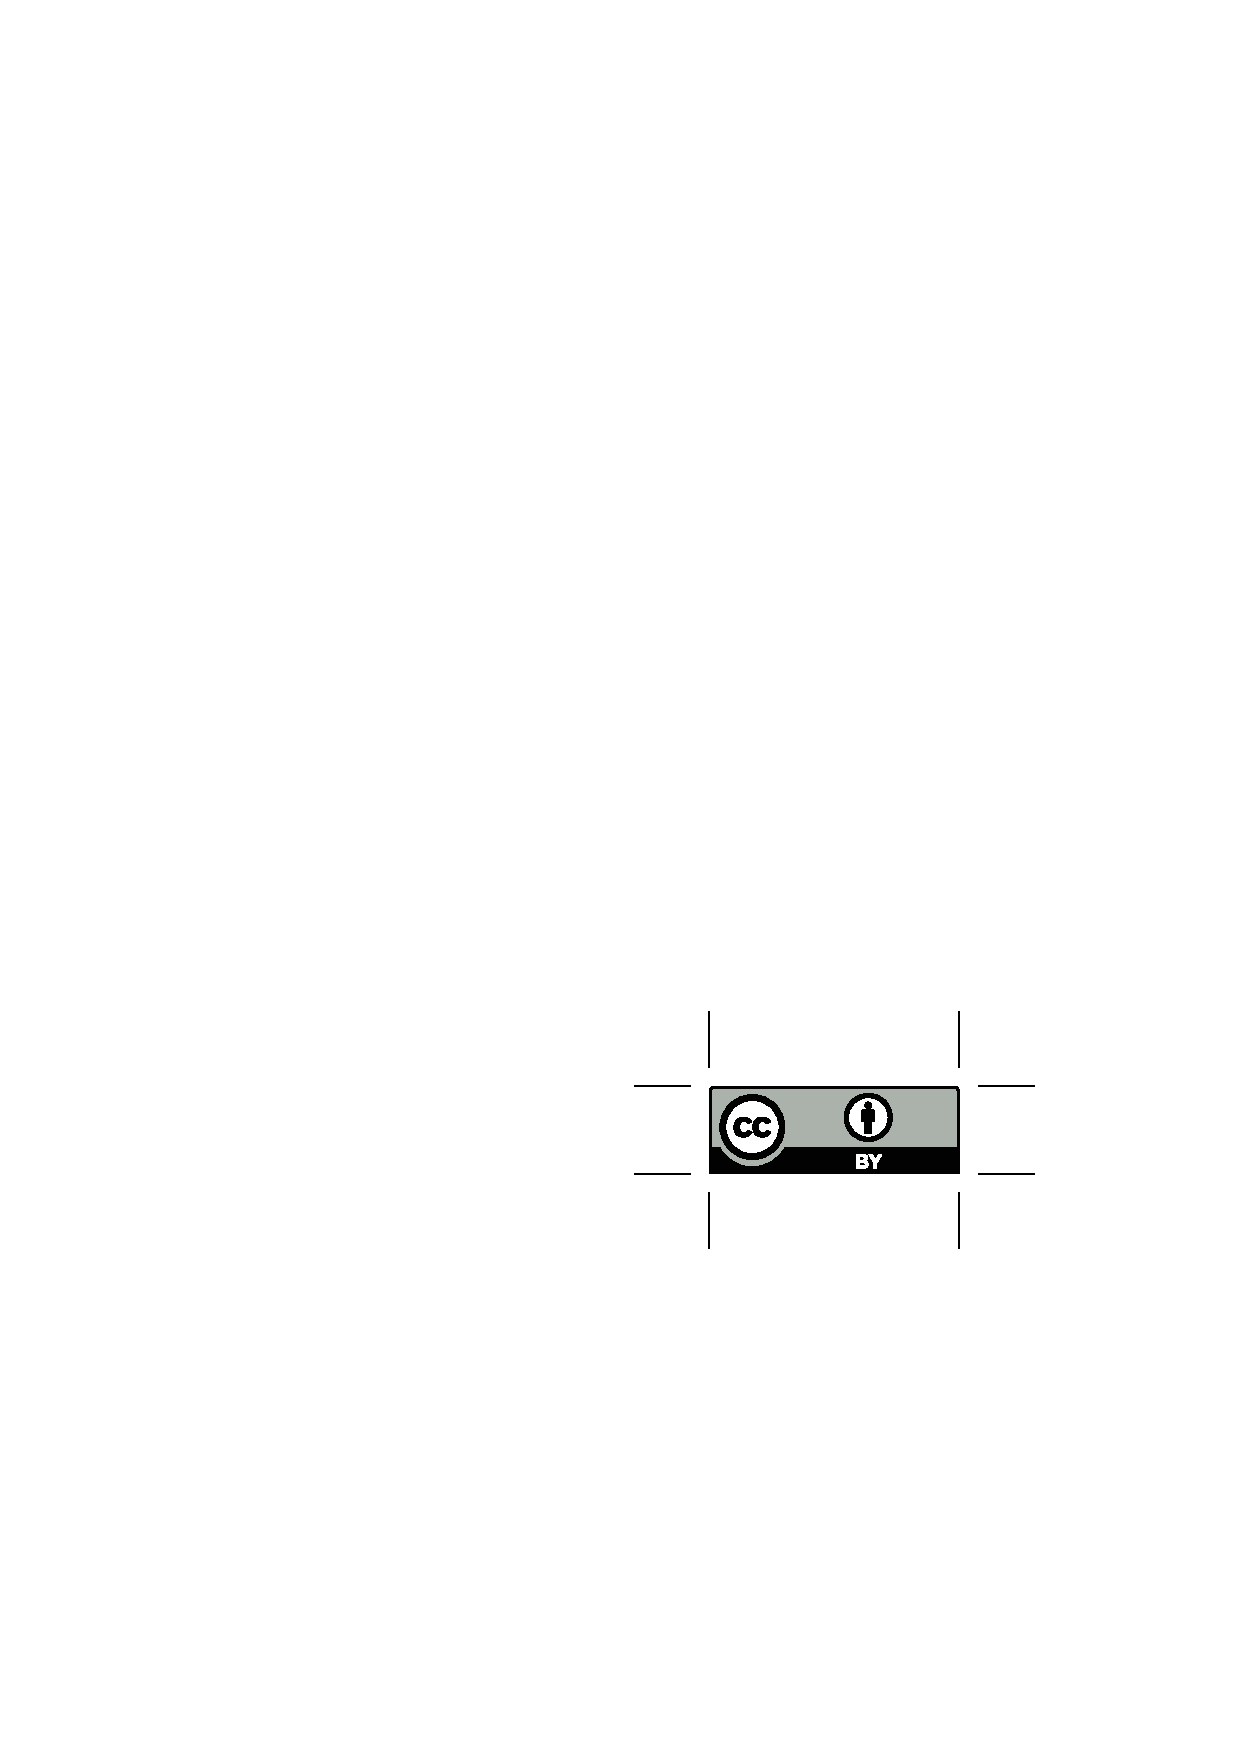
\includegraphics[width=0.90\textwidth]{by}}
  \end{minipage}\hfill
  \begin{minipage}{0.8\columnwidth}
   \href{https://creativecommons.org/licenses/by/4.0/}{This work is licensed under a Creative Commons Attribution International 4.0 License.}
  \end{minipage}
  \vspace{5pt}
}
\makeatother

\setcopyright{ifaamas}
\acmConference[AAMAS 2027]{Proc.\@ of the 26th International Conference
on Autonomous Agents and Multiagent Systems (AAMAS 2027)}{3--7 May 2027}{Hanoi, Vietnam}{M.~Baldoni, F.~Fang, W.~Yeoh, N.~Yorke-Smith (eds.)}
\copyrightyear{2027}
\acmYear{2027}
\acmDOI{}
\acmISBN{}

\acmSubmissionID{<<OpenReview submission id>>}
\submissionType{Research Paper Track}

%% Generated numbers (letters-only macro names).
% Generated by paper/AAMAS/analysis/selfplay.py. Do not edit by hand.
\newcommand{\CntGames}{3{,}950}
\newcommand{\CntGamesBaseline}{550}
\newcommand{\CntGamesNoCue}{150}
\newcommand{\CntGamesProbe}{150}
\newcommand{\CntGamesScripted}{1{,}000}
\newcommand{\CntGamesMixed}{1{,}500}
\newcommand{\CntGamesPara}{200}
\newcommand{\CntGamesTempZero}{100}
\newcommand{\CntGamesNeutral}{150}
\newcommand{\CntGamesWording}{150}
\newcommand{\CntDecisions}{187{,}000}
\newcommand{\CntParseFail}{2}
\newcommand{\CntReps}{10}
\newcommand{\LotMaxDraw}{0.47}
\newcommand{\LotRealCat}{96}
\newcommand{\LotExpCat}{69}
\newcommand{\GridZeroSeats}{300}
\newcommand{\GridZeroPaying}{240}
\newcommand{\GridZeroPayingPct}{80}
\newcommand{\GridZeroModelsPaying}{four}
\newcommand{\GridZeroModelsPayingCap}{Four}
\newcommand{\GridLossPanelPct}{42}
\newcommand{\GridGrokLossPct}{80}
\newcommand{\GridFlashLossPct}{21}
\newcommand{\GridQwenLossPct}{57}
\newcommand{\GridQwenReach}{2}
\newcommand{\GridQwenLastZeroPct}{95}
\newcommand{\GridQwenRoundsOneNinePct}{99}
\newcommand{\GridQwenFixReachPct}{100}
\newcommand{\GridGrokWaste}{13.0}
\newcommand{\GridGrokSecuredRound}{6.7}
\newcommand{\GridHaikuStopPct}{89}
\newcommand{\GridHaikuStopOtherPct}{12}
\newcommand{\GridFlashExactPct}{99.7}
\newcommand{\GridStepGrok}{4.4}
\newcommand{\GridStepMaxOther}{0.2}
\newcommand{\GridMissOnPace}{121}
\newcommand{\GridMissTotal}{121}
\newcommand{\GridLunaMiss}{23}
\newcommand{\GridLunaGames}{100}
\newcommand{\GridOptMean}{25.5}
\newcommand{\GridCrraLow}{0.85}
\newcommand{\NoCueQwenReachBase}{0}
\newcommand{\NoCueQwenReach}{100}
\newcommand{\NoCueQwenPayBase}{10.8}
\newcommand{\NoCueQwenPay}{5.2}
\newcommand{\NoCueGrokAllFourPct}{99}
\newcommand{\NoCueFlashExactPct}{97}
\newcommand{\NoCueLunaExactBasePct}{83}
\newcommand{\NoCueLunaExactPct}{56}
\newcommand{\NoCuePanelReachBase}{76}
\newcommand{\NoCuePanelReach}{91}
\newcommand{\NoCuePanelPayBase}{14.5}
\newcommand{\NoCuePanelPay}{12.1}
\newcommand{\RobGrokBase}{35.1}
\newcommand{\RobGrokParaTwo}{20.6}
\newcommand{\RobGrokParaTwoExactGames}{15}
\newcommand{\RobFlatMaxShift}{1.0}
\newcommand{\RobTempZeroDistinct}{5.5}
\newcommand{\RobTempZeroBaseDistinct}{6.6}
\newcommand{\RobGrokRiskBase}{6.2}
\newcommand{\RobGrokRiskParaTwo}{1.0}
\newcommand{\RobGrokRiskRerun}{1.9}
\newcommand{\RobQwenLastZeroBase}{97}
\newcommand{\RobQwenLastZeroNoHint}{41}
\newcommand{\RobQwenLastZeroParaOne}{57}
\newcommand{\RobQwenLastZeroParaTwo}{100}
\newcommand{\RobQwenLastZeroNeutral}{100}
\newcommand{\RobQwenLastZeroWording}{93}
\newcommand{\NeuZeroSeats}{300}
\newcommand{\NeuZeroPaying}{132}
\newcommand{\NeuZeroModelsPaying}{one}
\newcommand{\NeuZeroModelsPayingCap}{One}
\newcommand{\NeuZeroHaiku}{0.3}
\newcommand{\NeuStepHaiku}{0.4}
\newcommand{\NeuLowHaiku}{19.8}
\newcommand{\NeuHighHaiku}{20.2}
\newcommand{\NeuReachHaiku}{16}
\newcommand{\NeuGamesHaiku}{30}
\newcommand{\NeuZeroFlashLite}{1.4}
\newcommand{\NeuStepFlashLite}{$-$0.2}
\newcommand{\NeuLowFlashLite}{20.2}
\newcommand{\NeuHighFlashLite}{20.0}
\newcommand{\NeuReachFlashLite}{19}
\newcommand{\NeuGamesFlashLite}{30}
\newcommand{\NeuZeroLuna}{0.2}
\newcommand{\NeuStepLuna}{12.4}
\newcommand{\NeuLowLuna}{7.7}
\newcommand{\NeuHighLuna}{20.1}
\newcommand{\NeuReachLuna}{9}
\newcommand{\NeuGamesLuna}{30}
\newcommand{\NeuZeroQwen}{4.8}
\newcommand{\NeuStepQwen}{3.7}
\newcommand{\NeuLowQwen}{6.4}
\newcommand{\NeuHighQwen}{10.1}
\newcommand{\NeuReachQwen}{0}
\newcommand{\NeuGamesQwen}{30}
\newcommand{\NeuZeroGrok}{36.7}
\newcommand{\NeuStepGrok}{2.0}
\newcommand{\NeuLowGrok}{36.7}
\newcommand{\NeuHighGrok}{38.7}
\newcommand{\NeuReachGrok}{30}
\newcommand{\NeuGamesGrok}{30}
\newcommand{\WorZeroSeats}{300}
\newcommand{\WorZeroPaying}{245}
\newcommand{\WorZeroModelsPaying}{four}
\newcommand{\WorZeroModelsPayingCap}{Four}
\newcommand{\WorZeroHaiku}{18.0}
\newcommand{\WorStepHaiku}{0.3}
\newcommand{\WorLowHaiku}{20.9}
\newcommand{\WorHighHaiku}{21.2}
\newcommand{\WorReachHaiku}{25}
\newcommand{\WorGamesHaiku}{30}
\newcommand{\WorZeroFlashLite}{19.9}
\newcommand{\WorStepFlashLite}{0.0}
\newcommand{\WorLowFlashLite}{20.0}
\newcommand{\WorHighFlashLite}{20.0}
\newcommand{\WorReachFlashLite}{27}
\newcommand{\WorGamesFlashLite}{30}
\newcommand{\WorZeroLuna}{0.4}
\newcommand{\WorStepLuna}{0.0}
\newcommand{\WorLowLuna}{19.4}
\newcommand{\WorHighLuna}{19.4}
\newcommand{\WorReachLuna}{6}
\newcommand{\WorGamesLuna}{30}
\newcommand{\WorZeroQwen}{18.1}
\newcommand{\WorStepQwen}{$-$0.3}
\newcommand{\WorLowQwen}{18.9}
\newcommand{\WorHighQwen}{18.6}
\newcommand{\WorReachQwen}{1}
\newcommand{\WorGamesQwen}{30}
\newcommand{\WorZeroGrok}{39.8}
\newcommand{\WorStepGrok}{0.6}
\newcommand{\WorLowGrok}{39.4}
\newcommand{\WorHighGrok}{40.0}
\newcommand{\WorReachGrok}{30}
\newcommand{\WorGamesGrok}{30}
\newcommand{\GridZeroHaiku}{20.9}
\newcommand{\GridZeroFlashLite}{20.0}
\newcommand{\GridZeroLuna}{0.0}
\newcommand{\GridZeroQwen}{18.0}
\newcommand{\GridZeroGrok}{37.4}

% Generated by paper/AAMAS/analysis/probes.py. Do not edit by hand.
\newcommand{\ProbeGames}{150}
\newcommand{\ProbeQuestions}{4{,}500}
\newcommand{\ProbeRuleQuestions}{3{,}600}
\newcommand{\ProbeRulePct}{100}
\newcommand{\ProbeValueQuestions}{900}
\newcommand{\ProbeCorrectHaikuPct}{100}
\newcommand{\ProbeCorrectFlashPct}{99}
\newcommand{\ProbeCorrectLunaPct}{84}
\newcommand{\ProbeCorrectQwenPct}{33}
\newcommand{\ProbeCorrectGrokPct}{46}
\newcommand{\ProbeQwenKeepPct}{100}
\newcommand{\ProbeGrokRoundOneKeepPct}{100}
\newcommand{\ProbeThreeLowKeepPct}{97}
\newcommand{\ProbeThreeLowContrib}{20.1}
\newcommand{\ProbeThreeHighContrib}{20.3}
\newcommand{\ProbeThreeRiskShift}{0.3}
\newcommand{\ProbeThreeRiskShiftLo}{$-$0.5}
\newcommand{\ProbeThreeRiskShiftHi}{1.0}
\newcommand{\ProbeLunaSwitchGames}{13}

% Generated by paper/AAMAS/analysis/scripted.py. Do not edit by hand.
\newcommand{\ScrGames}{1{,}000}
\newcommand{\ScrDominatedGames}{500}
\newcommand{\ScrBestResponseDominated}{0}
\newcommand{\ScrMinTotalDominated}{2}
\newcommand{\ScrOptimalGames}{186}
\newcommand{\ScrOptimalAllTwenty}{every}
\newcommand{\ScrOpponentShareMin}{69}
\newcommand{\ScrOpponentShareMax}{92}
\newcommand{\ScrRiskShareMax}{5}
\newcommand{\ScrGrokOpponentShare}{3}
\newcommand{\ScrBestResponderRiskShare}{50}
\newcommand{\ScrWasteHaiku}{0.6}
\newcommand{\ScrWasteFlash}{0.1}
\newcommand{\ScrWasteLuna}{0.0}
\newcommand{\ScrCleanLuna}{100}
\newcommand{\ScrWasteQwen}{10.1}
\newcommand{\ScrCleanQwen}{0}
\newcommand{\ScrWasteGrok}{13.7}
\newcommand{\ScrCleanGrok}{1}
\newcommand{\ScrGrokRiskShare}{8}
\newcommand{\ScrGrokResidShare}{90}
\newcommand{\ScrQwenFairMiss}{47}
\newcommand{\ScrQwenFairShort}{2}
\newcommand{\ScrFlashFairReach}{50}
\newcommand{\ScrQwenDefectPay}{29.9}
\newcommand{\ScrQwenFairPay}{18.1}
\newcommand{\ScrFreeRiderGapMin}{3.7}
\newcommand{\ScrFreeRiderGapMax}{15.1}
\newcommand{\ScrGrokOpenFour}{103}
\newcommand{\ScrGrokFirstMoveShare}{74}
\newcommand{\ScrGrokProfileShareFour}{2}

% Generated by paper/AAMAS/analysis/mixed.py. Do not edit by hand.
\newcommand{\MixGames}{1{,}500}
\newcommand{\MixPairs}{10}
\newcommand{\MixFlashAloneReach}{100}
\newcommand{\MixFlashQwenReach}{11}
\newcommand{\MixLunaAloneReach}{78}
\newcommand{\MixLunaQwenReach}{9}
\newcommand{\MixHaikuQwenReach}{30}
\newcommand{\MixGrokQwenReach}{30}
\newcommand{\MixQwenPotZeroPct}{92}
\newcommand{\MixFlashPotZeroPct}{0.1}
\newcommand{\MixMissWithQwen}{323}
\newcommand{\MixMissTotal}{385}
\newcommand{\MixQwenPivotalFix}{92}
\newcommand{\MixLunaBesideFiveGrok}{10.5}
\newcommand{\MixLunaBesideOthers}{19.1}
\newcommand{\MixFlashBesideFiveGrok}{14.6}
\newcommand{\MixHaikuBesideFiveGrok}{16.1}
\newcommand{\MixLunaEarlyShort}{0.46}
\newcommand{\MixFlashEarlyShort}{0.04}
\newcommand{\MixHaikuEarlyShort}{0.03}
\newcommand{\MixGrokRescuesQwen}{25}
\newcommand{\MixHaikuRescuesQwen}{7}
\newcommand{\MixQwenBesideGrok}{20.8}
\newcommand{\MixQwenBesideOthers}{19.2}

% Generated by paper/AAMAS/analysis/selection.py. Do not edit by hand.
\newcommand{\SelIdentityMaxErr}{$<10^{-12}$}
\newcommand{\SelSignAgree}{1{,}500}
\newcommand{\SelGrokLosesCells}{12}
\newcommand{\SelQwenCells}{60}
\newcommand{\SelQwenBelowCells}{one}
\newcommand{\SelQwenAboveCells}{40}
\newcommand{\SelWithinQwenMassLow}{0.89}
\newcommand{\SelWithinQwenMassMid}{0.66}
\newcommand{\SelWithinQwenMassHigh}{0.47}
\newcommand{\SelWithinReachHigh}{47}
\newcommand{\SelWithinPayHigh}{10.6}
\newcommand{\SelAcrossFlashMassMid}{1.00}
\newcommand{\SelAcrossFlashMassHigh}{1.00}
\newcommand{\SelAcrossReachHigh}{100}
\newcommand{\SelAcrossPayHigh}{20.0}
\newcommand{\SelUniformReachHigh}{76}
\newcommand{\SelAcrossWinnerLow}{Qwen}
\newcommand{\SelSwitchN}{7}
\newcommand{\SelBootMinPct}{93}
\newcommand{\SelBetaExtra}{10}
\newcommand{\SelNExtra}{60 and 120}
\newcommand{\SelStrongWithinReachMid}{0}
\newcommand{\SelStrongWithinReachHigh}{1}
\newcommand{\SelWithinReachMid}{28}
\newcommand{\SelUniformReachMid}{75}
\newcommand{\SelWeakBeta}{0.1}
\newcommand{\SelWeakWithinMaxMass}{0.34}
\newcommand{\SelWeakAcrossTopHigh}{Gemini Flash-Lite}
\newcommand{\SelWeakAcrossTopMid}{Gemini Flash-Lite}

% Generated by paper/AAMAS/analysis/advantage.py. Do not edit by hand.
\newcommand{\AdvGrokWorst}{14.5}
\newcommand{\AdvGrokWorstPartner}{GPT-5.6 Luna}
\newcommand{\AdvQwenBest}{8.2}
\newcommand{\AdvQwenBestPartner}{Grok 4.20}
\newcommand{\AdvMaxAbs}{14.5}
\newcommand{\AdvPairLowReach}{13}
\newcommand{\AdvPairLowReachName}{Gemini 3.5 Flash-Lite and Qwen3-235B}
\newcommand{\AdvPairLowReachPct}{9}


\newcommand{\popt}{p^{*}}

\title{Cooperation by Default: LLM Agents in the Collective-Risk Dilemma}

\author{Anonymous Author(s)}
\affiliation{\institution{Anonymous Institution}\country{}}

\begin{abstract}
Language-model agents now act for people in shared settings, where one agent's choice can
put a whole group at risk. We ask whether such agents cooperate by weighing the risk and
their partners, or by default: play that does not change with what is at stake. In the
collective-risk social dilemma, six players pay into a shared pool over ten rounds, and if
the pool misses a target, everyone loses their savings with some probability. For
risk-neutral players, the best outcome is to keep the money at low risk and pay a fair share
at high risk. We test five low-cost models, one per provider, in almost four thousand games:
self-play across risk levels, prompt controls, scripted partners, and tables that mix two
models. Four models pay about the fair share at every positive risk level, and four of the
five still pay when there is no risk. Removing normative words from the prompt changes
neither result. Stating that only the agent's own cash matters largely stops three models
from paying at zero risk, but only one then keeps most of its money at low risk. Asked in a separate
call, several models rank the two choices correctly for each risk level, yet their payments
do not change. Beside scripted partners who make every payment a loss, no model pays
nothing, and two models keep paying after the outcome is settled. In mixed groups, one agent
that stops paying in the last round breaks a table of exact fair-share players. Under
selection by payoff, scoring agents against their tablemates rewards the smallest payer and
lowers group success, while scoring them across separate groups favours the fair-share
player at moderate and high risk. Agent evaluations should state the agent's goal, compare
play with the optimum and use mixed populations.
\end{abstract}

\keywords{LLM agents; collective-risk social dilemma; cooperation; best response;
empirical game-theoretic analysis; multiagent evaluation}

\begin{document}

\maketitle

%% =====================================================================================
%% 1 Introduction. Spine of the paper, three sentences:
%%   believed: LLM agents that reach cooperative outcomes are cooperating strategically;
%%   found:    when the prompt leaves the agent's goal unstated, the models pay by default
%%             (play that does not follow the stakes, visible where paying cannot help);
%%             removing normative words keeps the default, stating the goal switches most
%%             of it off without making the models weigh the risk; defaults respond to
%%             partners only in simple ways and fail predictably in mixed groups and under
%%             selection;
%%   change:   state the agent's goal, evaluate against the optimum, in mixed populations,
%%             and choose the selection signal with care.
%% Scope rule: claims are about the five low-cost models tested, not about "LLMs".
%% Model names: always with the family (Claude Haiku, Gemini Flash-Lite, GPT Luna, Qwen,
%% Grok); a bare "Luna" does not tell the reader it is a GPT model.
%% =====================================================================================
\section{Introduction}
\label{sec:intro}
%% =====================================================================================
%% Overview figure (figure*, text width). Drawn by analysis/overview.py from the counts in
%% tables/num_selfplay.tex; placed right after \label{sec:intro} so it floats to page 2.
%% =====================================================================================
\begin{figure*}[t]
\centering
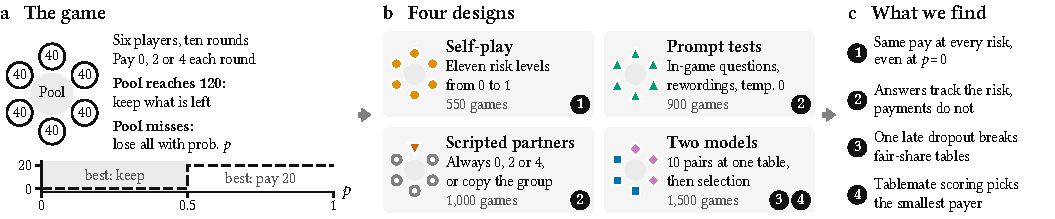
\includegraphics[width=\textwidth]{figures/fig_overview.pdf}
\Description{A three-part overview read from left to right. First, the game: six seats, each
holding 40 units, sit around a shared pool; each round a seat pays 0, 2 or 4, and a small
step plot shows that the best total per seat is 0 below catastrophe probability one half and
20 above it. Second, four design cards, each with a small table of model markers and a game
count: self-play on eleven risk levels, prompt tests, one model beside scripted partners, and
two models at one table followed by selection. Third, four numbered findings that match
numbered badges on the cards.}
\caption{Overview. (a)~Six players hold 40 units and pay 0, 2 or 4 into a shared pool in each
of ten rounds; if the pool misses 120, all savings are lost with probability $p$. Below: the
best total per seat (Proposition~\ref{prop:eq}). (b)~The designs, who sits at each table, and
the number of games. (c)~The findings; badges mark the design behind each.}
\label{fig:overview}
\end{figure*}


Language-model agents are starting to act for people in shared settings: they spend
budgets, share compute, and bargain over common resources. Each such agent is a player in a
social dilemma, because what it pays helps the group and costs its owner. Before deploying
one, a designer needs answers to two questions. Does the agent's cooperation depend on what
is at stake? And does it depend on what the other agents do?

Self-play, the most common test, cannot answer either question. When every seat holds a copy
of the same model, an agent that reasons about the stakes and an agent that repeats a fixed
rule can write the same record of play. Many studies also report whether the group reached
its goal, not how far the agents were from the best they could have done. Yet a group of
agents can reach its goal and still waste most of its money. Finally, a prompt that gives a
group target and a number of rounds implies an equal split, so an agent that repeats that
split looks cooperative on every summary measure.

We study these questions in a classic game from research on climate cooperation, the
collective-risk social dilemma~\cite{milinski2008collective}. Six players pay into a shared
pool over ten rounds, and if the pool misses a target, a catastrophe destroys everyone's
savings with probability $p$. For risk-neutral players, nobody should pay below a pivot
$\popt=\tfrac12$, and above it everyone should pay the \emph{fair share}, the target split
equally, which is half of each player's money. At $p=0$ paying only lowers a player's own
money, so no attitude to risk can explain it.

We call play a \emph{default} when it does not change with what is at stake. The game gives
two sharp tests of a default, because in both paying cannot help: paying at $p=0$, and
paying after the outcome can no longer change. We test five low-cost production models, one
per provider, in \CntGames{} games and four designs: self-play across eleven risk levels;
prompt controls, including questions about which choice pays more and prompts that remove
normative words or state the agent's goal; one model against five scripted partners, where
the best response can be computed exactly; and two different models at one table, which lets
us ask which agent would win if agents were selected by
payoff~\cite{wellman2006methods,tuyls2018generalised}. Our findings are four
(Figure~\ref{fig:overview}).

\begin{itemize}
\item \textbf{Risk does not change the default} (Section~\ref{sec:risk}). Four models pay
  about the fair share at every positive risk level, and four of five still pay at $p=0$.
  Removing the normative words from the prompt changes neither result. Stating that only
  the agent's own cash matters largely stops three models from paying at $p=0$, but only
  GPT Luna then switches from keeping its money at low risk to paying at high risk. Success
  rates hide the failures that remain.
\item \textbf{Answers track the risk; play does not} (Section~\ref{sec:knowing}). In
  separate calls, several models rank the two choices correctly and change that ranking with
  the risk, but they pay the same amount. Beside scripted partners who make every payment a
  loss, no model pays nothing, and two models keep paying after the outcome is settled.
\item \textbf{An exact fair share has no slack} (Section~\ref{sec:groups}). One partner
  that stops paying in the last round breaks a table of exact fair-share players, while a
  table that overpays a little absorbs it. Agents pay less when generous partners fill most
  of the table.
\item \textbf{The scoring rule decides who is selected} (Section~\ref{sec:selection}).
  Seats at one table share the pool and the lottery, so the smaller payer always earns more
  there. Scoring agents against their tablemates therefore favours the smallest payer and,
  in our games, lowers group success. Scoring them across separate groups favours the exact
  fair-share player at moderate and high risk.
\end{itemize}

For the models we test, cooperation is a default that follows from what the prompt leaves
unsaid, not a choice that follows from the stakes. A default can work well beside partners
like itself, but it cannot be trusted with shared resources, and the way a system states
its agents' goals and selects its agents can make the problem better or worse.

%% =====================================================================================
%% 2 Related work. Each paragraph ends with how this paper differs.
%% The last paragraph declares the overlap with a concurrent manuscript. It is required
%% by the dual-submission policy; do not cut it to save space. Cite it in the third
%% person only (double-blind).
%% Claims about other papers were checked against their full text on 2026-09-16.
%% =====================================================================================
\section{Related work}
\label{sec:related}

\paragraph{Collective risk and selection.}
The collective-risk dilemma was built to study why groups fail to avoid a shared
disaster~\cite{milinski2008collective}. Human groups reach the target mostly when the risk
is high, and inequality and communication change the result~\cite{tavoni2011inequality}.
Games with a threshold have many equilibria~\cite{palfrey1984participation}, human
contributions decline over the rounds of repeated public goods games~\cite{andreoni1988free},
and the risk of collective failure can turn a defection trap into a coordination
problem~\cite{santos2011risk}. Theory also shows that selection on payoff relative to a small
group favours whoever does better than its neighbours~\cite{schaffer1988evolutionarily},
while selection between groups can favour cooperation~\cite{traulsen2006evolution}. This
literature tells us that behaviour \emph{should} move with the risk, so a flat response is
informative, and we reuse its selection theory to read our mixed tables.

\paragraph{Language models in games.}
Language models have been studied as economic
subjects~\cite{horton2023large,chen2023emergence,mei2024turing}, in repeated two-player
games~\cite{akata2025playing,fontana2024nicer}, and in multi-player game
benchmarks~\cite{huang2025competing}. Models tend to be more cooperative than
people~\cite{mei2024turing}, an even split can reflect a focal point rather than
fairness~\cite{dodivers2025uncovering}, and models can hold a correct belief or plan and act
against it~\cite{fan2024can,schmied2026llms}. In social dilemmas, societies of agents
over-use a common resource~\cite{piatti2024cooperate}, reasoning models free-ride in public
goods games~\cite{guzmanpiedrahita2025corrupted}, and agents replace people in a
collective-risk game~\cite{slumbers2025using}. Closest to us, Willis et al.\ study the same
collective-risk game with strategies written by three models, map welfare over mixtures of
selfish and collective strategies, and find that payoff-biased imitation drives larger
groups to selfish, low-welfare outcomes~\cite{willis2026evaluating}. We differ in three ways.
We record the turn-by-turn play of deployed models, not code they write. We price that play
against a computed optimum, with two tests where paying cannot help. And we show that
whether selection compares tablemates or separate groups decides which model wins, which
gives one simple route to selfish outcomes.

\paragraph{Multiagent evaluation.}
Sequential social dilemmas made cooperation a property of learned
policies~\cite{leibo2017multi,hughes2018inequity}, and cooperative AI asks for agents that
work with partners unlike themselves~\cite{dafoe2020open,stone2010ad}. Melting Pot tests a
focal population against background agents it has never met~\cite{leibo2021scalable}.
Empirical game-theoretic analysis treats trained agents as strategies of a
meta-game~\cite{wellman2006methods,tuyls2018generalised}, and $\alpha$-Rank ranks them by
evolutionary dynamics~\cite{omidshafiei2019alpha}. Tournaments that mix language models with
classic strategies report model-specific strategic fingerprints in the prisoner's
dilemma~\cite{payne2025strategic}, and cooperation evolves differently across base models in
a donor game~\cite{vallinder2025cultural}. We add a many-player dilemma in which the best
response to fixed partners can be computed exactly, and real tables of two different models.

\paragraph{Overlap with concurrent work.}
A concurrent manuscript uses the same game and an overlapping set of models to ask whether
models reproduce the risk sensitivity of human players, and suggests that more capable models
can respond to risk~\cite{anon-if}. It reports a self-play risk baseline related to part of
Section~\ref{sec:risk}. The present paper asks how low-cost agents behave against the
optimum, against fixed partners and against other models; the tests where paying cannot
help and Sections~\ref{sec:knowing} to~\ref{sec:selection} have no counterpart there.

%% =====================================================================================
%% 3 Game, benchmarks, designs.
%% Proposition 1 is checked by exhaustive search in crsd/tests/test_paper_equilibrium.py
%% (all symmetric profiles plus 6,000 asymmetric ones at 11 risk levels). If you change
%% the statement, change the test. p = 1 is excluded on purpose: at p = 1 every profile
%% that misses the target is a weak equilibrium.
%% The verbatim prompts (base, no hint, neutral wording, goal stated, two rewordings) live
%% in supplement/supplement.tex, rendered from kaggle/benchmarks/crg_task_server.py. The
%% Prompts paragraph below must quote exactly the spans each condition changes.
%% =====================================================================================
\section{The game and what rational play looks like}
\label{sec:game}

\subsection{Rules}
Six players each start with $e=40$ units. A \emph{seat} is one player position and a
\emph{table} is the six seats of one game. In each of $R=10$ rounds, every player privately
chooses a contribution $a_i^t\in\{0,2,4\}$ to a shared \emph{pool}; after each round all
players see every seat's past contributions. Let $x_i=\sum_t a_i^t$ be a player's total and
$X=\sum_i x_i$ the pool. The target is $T=120$. A player keeps what it did not pay, but if
the pool misses the target a catastrophe destroys all savings with probability $p$:
\begin{equation}
u_i \;=\;
\begin{cases}
e-x_i & \text{if } X\ge T,\\
0 \text{ with probability } p, \text{ else } e-x_i & \text{if } X<T.
\end{cases}
\label{eq:payoff}
\end{equation}
The fair share is $T/6=20$ per player, or 2 per round.

\begin{proposition}
\label{prop:eq}
Consider the game in which each player picks a total $x_i\in\{0,2,\dots,40\}$, and let
$p<1$. A profile is a Nash equilibrium if and only if $x=0$, or $X=T$ and $x_i\le pe$ for
every $i$. A target-reaching equilibrium exists if and only if $p\ge\popt=T/(6e)=\tfrac12$.
The welfare-optimal outcome is $x=0$ for $p<\popt$ and $X=T$ for $p>\popt$, so the best
attainable payoff per player is $\mathrm{opt}(p)=\max\{(1-p)e,\;e-T/6\}$.
\end{proposition}

\noindent\emph{Proof sketch.} If $X<T$, any player with $x_i>0$ gains by paying nothing, so
the only equilibrium that misses the target is $x=0$. If $X>T$, a player can pay 2 less and
still reach the target. If $X=T$, the best deviation is to pay nothing, worth $(1-p)e$
against $e-x_i$, which gives $x_i\le pe$; summing over players gives $p\ge T/(6e)$. Welfare
is $6e-X$ when the target is met and $(1-p)(6e-X)$ otherwise, so it peaks at $X=T$ or
$X=0$.\hfill$\square$

The ten-round game, whose strategies can react to the history, has the same totals in
pure-strategy Nash equilibrium; we claim nothing about subgame perfection. Paying nothing
in every round secures $(1-p)e$ whatever the others do, so no equilibrium misses the target
with $x\neq0$ or has $x_i>pe$. A payment
beyond the target can be dropped in the round the target is reached, or later, and nothing
played afterwards can lower that player's payoff. Each profile of
Proposition~\ref{prop:eq} is played by fixed schedules that ignore the history.

Three benchmarks follow and carry the rest of the paper. First, the \emph{optimum}, the
welfare optimum for risk-neutral players, switches at $\popt$, as does the best response to
five fair-share partners; it is a benchmark, not a prediction, since $x=0$ is an equilibrium
at every $p$. Second, paying is
\emph{dominated}, meaning that every unit paid lowers the seat's own payoff whatever else
happens, in two situations: at $p=0$, where both branches of \eqref{eq:payoff} are equal,
and once the outcome is \emph{settled}, meaning that the visible history already proves that
more payment cannot change it (the pool has reached the target, or cannot reach it even if
every seat pays 4 in every remaining round). Neither test depends on the agent's attitude to
risk or on its beliefs. Third, these two tests are the sharpest evidence of a default:
payment that continues where paying is dominated cannot follow from the stakes.

\begin{proposition}
\label{prop:table}
For two seats $i$ and $j$ in the same game, the difference in their expected payoffs over
the lottery is $c\,(x_j-x_i)$, with $c=1$ if the target was reached and $c=1-p$ otherwise.
\end{proposition}

\noindent Both seats face the same pool and the same lottery, so only their own payments
differ. Hence, for $p<1$, whoever pays less at a table earns more, whatever the group
achieves.

\subsection{Models, designs and measures}

We test five production models, one per provider, all at the low-cost tier of their family:
Claude Haiku 4.5 (Anthropic), Gemini 3.5 Flash-Lite (Google), GPT-5.6 Luna (OpenAI),
Qwen3-235B-A22B-Instruct (Alibaba) and Grok 4.20 in its non-reasoning mode (xAI). We call
them Claude Haiku, Gemini Flash-Lite, GPT Luna, Qwen and Grok; the supplementary material
gives the exact model identifiers. We chose this tier because agents that act at scale are
likely to run on it. Table~\ref{tab:designs} lists the designs. Every model plays the same
number of games in every design, and every cell holds \CntReps{} games.

\begin{table}[t]
\caption{Designs. A cell is one condition at one risk level: one model in self-play, one
model with one kind of script, or one pair of models with one split of seats. Each cell holds
ten games. The in-game question condition uses the unchanged prompt, so it also repeats the
self-play grid at three risk levels.}
\label{tab:designs}
\small
\setlength{\tabcolsep}{3pt}
\begin{tabular}{llr}
\toprule
Design & Risk levels $p$ & Games \\
\midrule
Self-play grid & $0, 0.1, \dots, 1$ & \CntGamesBaseline \\
In-game questions & $0.1, 0.5, 0.9$ & \CntGamesProbe \\
No hint & $0.1, 0.5, 0.9$ & \CntGamesNoCue \\
Neutral wording & $0, 0.1, 0.9$ & \CntGamesWording \\
Neutral wording, goal stated & $0, 0.1, 0.9$ & \CntGamesNeutral \\
Two rewordings & $0.1, 0.9$ & \CntGamesPara \\
Temperature zero & $0.1, 0.9$ & \CntGamesTempZero \\
One model, five scripts (4 kinds) & $0.1, 0.3, \dots, 0.9$ & \CntGamesScripted \\
Two models (10 pairs, 1 to 5 seats) & $0.1, 0.5, 0.9$ & \CntGamesMixed \\
\midrule
All & & \CntGames \\
\bottomrule
\end{tabular}
\end{table}

\paragraph{Prompts.}
Each round a seat receives one prompt: the rules, the full history of every seat's
contributions, and a request for one contribution. The supplementary material gives every
prompt verbatim. The base prompt calls the pool a ``climate account'', says that the group
``must'' reach the target, calls the loss a ``disaster'', names the game as a collective-risk
social dilemma, and never states the player's goal. It also states the equal split twice, as
an average of 2 per round and as an example in which paying 2 every round leaves 20. The
prompt controls change exactly these parts. \emph{No hint} deletes the two equal-split
phrases. \emph{Neutral wording} replaces the four normative or naming phrases with plain
ones, such as ``a shared account'' and ``the outcome depends on whether'' the pool reaches
120. \emph{Goal stated} keeps the neutral wording and adds an opening that says the player
is in a paid experiment where ``the only thing that matters to you is your own final cash
payoff''. Two \emph{rewordings} change the phrasing but keep every rule and the hint.

\paragraph{Protocol.}
The running pool is not printed, so a seat that wants it must add up the history. The
prompt is in English, no seat
is given a persona, and the temperature is 0.7 unless stated. A reply is read from its final
\texttt{CONTRIBUTION:} line; replies cut off at the output limit are retried with a larger
limit rather than guessed. The data contain \CntDecisions{} model decisions. Only
\CntParseFail{} replies could not be read, and both come from one reworded prompt.

\paragraph{Measures.}
We report the \emph{expected} payoff, the average a seat would earn if the catastrophe
lottery were run many times on the same contributions, and the share of $\mathrm{opt}(p)$ it
loses. We do not use realised payoffs. A catastrophe strikes when a uniform random draw falls
below $p$, and the draw depends only on the repetition number, so our games reuse ten draws in
every cell, all below \LotMaxDraw{}. Every missed game at $p\ge\popt$ therefore ended in
catastrophe, and realised payoffs would punish models that miss more than chance would.
Agents never see the draw, so their play is not affected. A seat plays the \emph{exact split}
if it pays 2 in all ten rounds. The unit of analysis is the game, since seats in one game
share a history and a lottery. Intervals are 95\% percentile bootstraps over games and tests
are permutation tests over games.

%% =====================================================================================
%% 4 Self-play across risk, plus prompt and decoding controls.
%% Numbers: tables/num_selfplay.tex (analysis/selfplay.py). Figure: fig_selfplay.pdf.
%% Tables: tab_models.tex, tab_robust.tex (tabular only; captions live here).
%% =====================================================================================
\section{Risk does not change the default}
\label{sec:risk}

\begin{figure*}[t]
\centering
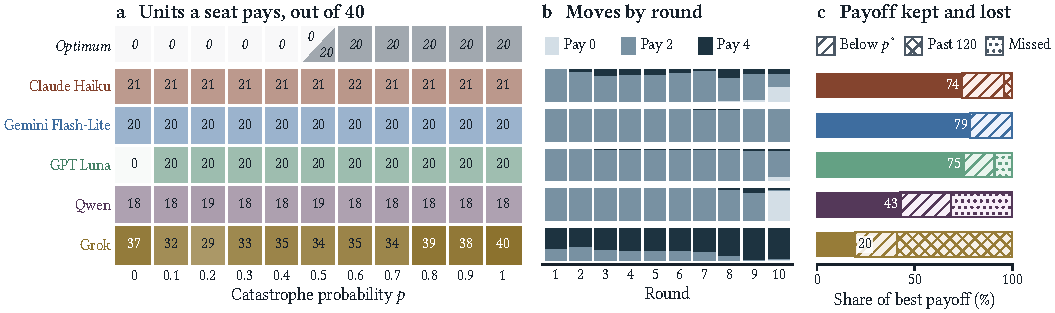
\includegraphics[width=\textwidth]{figures/fig_selfplay.pdf}
\Description{Three panels that share one row per model, below a reference row. Left: a grid
of the mean units a seat pays at each catastrophe probability from 0 to 1. The optimum row
switches from 0 to 20 at one half, while the model rows barely change: about 20 for four
models, 0 only for GPT Luna at probability zero, and 29 to 40 for Grok. Middle: for each round,
the share of seats paying 0, 2 or 4; Qwen pays 2 until round 10 and then almost always 0, and
Grok mostly pays 4. Right: bars of the share of the best attainable payoff each model keeps;
Grok keeps about a fifth and loses most by paying past the target, and Qwen loses most by
missing it.}
\caption{Self-play on the risk grid, 110 games per model. (a)~Mean units a seat pays out of
40, ten games per cell; the top row is the optimum of Proposition~\ref{prop:eq}, where both 0
and 20 are optimal at $p=0.5$. (b)~Share of seats paying 0, 2 or 4 in each round, over the
100 games with $p>0$. (c)~Expected payoff kept as a share of $\mathrm{opt}(p)$, and the loss
split into paying toward the target below $\popt$, paying past 120, and missing the target at
or above $\popt$.}
\label{fig:selfplay}
\end{figure*}

Four of the five models pay about the fair share at every positive risk level
(Figure~\ref{fig:selfplay}). For Claude Haiku, Gemini Flash-Lite, GPT Luna and Qwen, the mean
total below the pivot and the mean total above it differ by at most \GridStepMaxOther{}
units, while a risk-neutral player would jump from 0 to 20. Risk aversion does not explain
the flat line either: preferring a certain 20 to keeping 40 with probability 0.9 requires a
coefficient of relative risk aversion of at least \GridCrraLow{}. Gemini Flash-Lite is the
clearest case: \GridFlashExactPct\% of its seats play the exact split at every risk level, so
its play is optimal above the pivot only because a fixed rule matches the optimum there.

\paragraph{Paying when there is nothing to protect.}
\GridZeroModelsPayingCap{} of the five models pay at $p=0$, close to their usual amount,
although paying there only lowers a player's own money (\GridZeroPaying{} of
\GridZeroSeats{} seats pay). GPT Luna is the one exception: it pays nothing at $p=0$ and its
usual share at every positive risk, so it separates no risk from some risk but does not
grade the risk.

\paragraph{Three ways to lose.}
The models lose payoff in three ways (Table~\ref{tab:models}). Gemini Flash-Lite, Claude
Haiku and GPT Luna lose mostly below the pivot, where they pay for a target that is not worth
reaching. Grok pays far more than needed: its groups reach the target by round
\GridGrokSecuredRound{} on average, and each seat then pays another \GridGrokWaste{} units
into a pool that is already safe. Qwen fails at the end. It pays 2 in
\GridQwenRoundsOneNinePct\% of decisions in rounds 1 to 9 and then \GridQwenLastZeroPct\% of
its seats pay nothing in round 10, so its groups reach the target in only \GridQwenReach{} of
110 games; had each seat repeated its round-9 move, \GridQwenFixReachPct\% would have
succeeded. This is a coordination failure, not one bad move: with 108 in the pool before
round 10, one seat alone can add at most 4, so paying nothing is also an equilibrium of that
round, and Qwen seats almost always pick it, much as human contributions decline at the end
of repeated public goods games~\cite{andreoni1988free}. GPT Luna shows a milder form: its
groups miss the target in \GridLunaMiss{} of \GridLunaGames{} games with $p>0$, always after
keeping pace until the last round. Claude Haiku shows that the pool can be read from the same
prompt: it pays nothing in round 10 in \GridHaikuStopPct\% of seats once the pool has reached
the target, against \GridHaikuStopOtherPct\% when it has not. Success rates hide all of this.
Gemini Flash-Lite and Grok both reach the target in every game, yet Grok keeps a quarter as
much money, and the panel loses \GridLossPanelPct\% of the attainable payoff.

\begin{table}[t]
\caption{Self-play summary over the risk grid, using expected payoffs. \emph{Pays at
$p{=}0$} is the mean seat total where paying is dominated. \emph{Exact split} is the share of
seats paying 2 in all ten rounds. \emph{Target} is the share of games that reach it, and
\emph{Payoff} is the expected payoff per seat; the optimum averages \GridOptMean{} over the
grid. \emph{Lost} is the share of the attainable payoff $\mathrm{opt}(p)$ that was lost, and
\emph{Main loss} is its largest cause: paying toward the target below $\popt$, paying beyond
120, or missing the target at or above $\popt$, which for Qwen happens in the last round.}
\label{tab:models}
% Generated by paper/AAMAS/analysis/selfplay.py. Do not edit by hand.
\begin{tabular}{@{}l@{\hspace{3pt}}r@{\hspace{3pt}}r@{\hspace{3pt}}r@{\hspace{3pt}}r@{\hspace{3pt}}r@{\hspace{3pt}}l@{}}
\toprule
 & Pays at & Exact & Target & Payoff & Lost & Main \\
Model & $p{=}0$ & split (\%) & (\%) & & (\%) & loss \\
\midrule
Claude Haiku & 20.9 & 17 & 98 & 18.9 & 26 & below $p^*$ \\
Gemini Flash-Lite & 20.0 & 99.7 & 100 & 20.0 & 21 & below $p^*$ \\
GPT Luna & 0.0 & 72 & 70 & 19.2 & 25 & below $p^*$ \\
Qwen & 18.0 & 4 & 2 & 10.9 & 57 & last round \\
Grok & 37.4 & 2 & 100 & 5.0 & 80 & overshoot \\
\bottomrule
\end{tabular}

\end{table}

\paragraph{The default survives rewording, but its failures do not.}
Deleting the two equal-split phrases does not lower anyone's payment
(Table~\ref{tab:robust}), so the hint was a ceiling and a guide for precision, not the source
of the cooperation. Gemini Flash-Lite still plays the exact split, which it can rebuild from
the target, and GPT Luna keeps its average but not its precision (the exact split falls from
\NoCueLunaExactBasePct\% to \NoCueLunaExactPct\% of seats). Qwen and Grok pay more; Qwen now
reaches the target in \NoCueQwenReach\% of games instead of \NoCueQwenReachBase\%, but earns
less because it overpays. Two rewordings and a temperature of zero leave the mean payments of
the other four models within \RobFlatMaxShift{} unit of the grid. The failures are less stable
than the means: under the second rewording Grok pays the fair share, and the share of Qwen
seats that pay nothing in round 10 ranges from \RobQwenLastZeroNoHint\% to
\RobQwenLastZeroParaTwo\% across prompts. Grok's rise with risk on the grid
(\RobGrokRiskBase{} units) shrinks to \RobGrokRiskRerun{} in the rerun, so we do not read it
as a response to risk.

\paragraph{Stating the goal, not removing the norms, switches the default off.}
The default does not come from the normative words. With the neutral wording,
\WorZeroModelsPaying{} models still pay at $p=0$ (\WorZeroPaying{} of \WorZeroSeats{} seats
pay), and at $p=0.1$ and $p=0.9$ four models pay what they paid before while Grok pays even
more (Table~\ref{tab:robust}). Adding the stated goal changes play at zero risk: Claude Haiku,
Gemini Flash-Lite and Qwen then pay \NeuZeroHaiku{}, \NeuZeroFlashLite{} and \NeuZeroQwen{}
units at $p=0$, against \GridZeroHaiku{}, \GridZeroFlashLite{} and \GridZeroQwen{} with the
base prompt. The goal does not make most models weigh the risk. Claude Haiku and Gemini
Flash-Lite still pay the fair share at $p=0.1$ (\NeuLowHaiku{} and \NeuLowFlashLite{} units),
so they separate no risk from some risk but do not grade it. GPT Luna alone grades it, paying
\NeuLowLuna{} units at $p=0.1$ and \NeuHighLuna{} at $p=0.9$. Qwen pays less at every level
and reaches the target in \NeuReachQwen{} of \NeuGamesQwen{} games, and Grok keeps paying far
more than needed. The default is therefore what these models do when the prompt leaves their
goal unstated; the scripted and mixed designs below use the base prompt and describe it.

\begin{table}[t]
\caption{Mean seat total under prompt and decoding changes, pooled over $p=0.1$ and $0.9$
(20 games per entry). \emph{Base} is the self-play grid. \emph{Rerun} is the in-game
question condition, which uses the unchanged prompt and was collected with the other
changes. \emph{No hint} deletes the equal-split phrases, \emph{Para.\,1} and \emph{Para.\,2}
are the two rewordings, \emph{Temp.\,0} sets the temperature to zero, \emph{Wording} uses the
neutral wording, and \emph{Neutral} adds the stated goal to it. Bold marks a shift from
\emph{Base} of at least 2 units with permutation $P<0.01$. Temperature zero was not
deterministic: a cell produced \RobTempZeroDistinct{} distinct games in ten, against
\RobTempZeroBaseDistinct{} at 0.7.}
\label{tab:robust}
% Generated by paper/AAMAS/analysis/selfplay.py. Do not edit by hand.
\begin{tabular}{@{}lrrrrr@{}}
\toprule
 & Claude & Gemini & GPT &  &  \\
Condition & Haiku & Flash-Lite & Luna & Qwen & Grok \\
\midrule
Base & 20.9 & 20.0 & 19.9 & 18.4 & 35.1 \\
Rerun & 21.3 & 20.0 & 19.9 & 18.5 & 35.6 \\
No hint & 21.7 & 20.0 & 19.9 & \textbf{34.7} & \textbf{40.0} \\
Para.\,1 & 21.3 & 20.0 & 19.9 & 19.4 & 31.8 \\
Para.\,2 & 20.9 & 20.0 & 19.8 & 18.0 & \textbf{20.6} \\
Temp.\,0 & 21.2 & 20.0 & 20.0 & 18.3 & 35.1 \\
Wording & 21.0 & 20.0 & 19.4 & 18.7 & \textbf{39.7} \\
Neutral & 20.0 & 20.1 & \textbf{13.9} & \textbf{8.2} & 37.7 \\
\bottomrule
\end{tabular}

\end{table}

%% =====================================================================================
%% 5 In-game questions and scripted partners.
%% Numbers: tables/num_probes.tex (analysis/probes.py), tables/num_scripted.tex and
%% tables/tab_settled.tex (analysis/scripted.py). Figures: fig_knowdo.pdf, fig_scripted.pdf.
%% Wording rule: probe answers come from separate calls that never enter the game, so
%% the claim is a dissociation between answers and play, never that an answer "causes"
%% or "fails to cause" an action.
%% =====================================================================================
\section{Answers track the risk; play does not}
\label{sec:knowing}

A flat response to risk has a cheap explanation: perhaps the agents do not understand the
game. We test this in two ways. We ask the playing agent which choice pays more, and we seat
it with partners whose behaviour is fixed, so that the \emph{best response}, the play that
earns the most against them, can be computed exactly.

\subsection{Asking the agent}

In \CntGamesProbe{} games we question the first seat in rounds 1, 5 and 10, on the state it
has just decided on. Each question is a separate call, and its answer never enters the game.
Of the \ProbeQuestions{} questions, \ProbeRuleQuestions{} ask about the rules, such as the
target or the allowed amounts. Agents answer \ProbeRulePct\% of them correctly, but these
questions only ask for numbers printed in the prompt, so they show that agents read the
rules, not that they understand them. We therefore rest on one value question, asked
verbatim:
\begin{quote}\small
\emph{Compare two strategies for the whole game. (A) You contribute 2 in every one of the 10
rounds and the group reaches the target, so you finish with 20 for certain. (B) You
contribute 0 in every round and the group does not reach the target, so you keep 40 unless
the disaster strikes. Which gives the higher AVERAGE final cash? Answer 1 if A is higher, 2
if B is higher, 0 if they are exactly equal.}
\end{quote}
The correct answer is B below $\popt$, A above it, and equal at $\popt$. A second value
question could be read in two ways and is not used.

\begin{figure}[t]
\centering
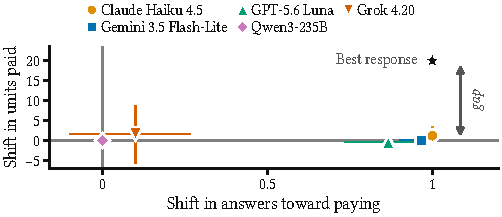
\includegraphics[width=\columnwidth]{figures/fig_knowdo.pdf}
\Description{A scatter plot with one point per model and 95 percent interval bars. The
horizontal axis is how far the model's answers move toward paying between catastrophe
probability 0.1 and 0.9; the vertical axis is how far its payment moves. Claude Haiku, Gemini
Flash-Lite and GPT Luna sit near 1 on the horizontal axis but near 0 on the vertical axis, far
below a star at 20 that marks the best response. Qwen sits at the origin and Grok close to
it.}
\caption{What agents say and do, from $p=0.1$ to $p=0.9$ in the same games (ten at each),
with 95\% intervals. Horizontal: drop in the share of answers saying that paying nothing pays
more on average; a correct answerer moves by 1. Vertical: change in what the questioned seat
pays. Star: a best responder beside fair-share partners.}
\label{fig:knowdo}
\end{figure}

\paragraph{Answers move with the risk; play does not.}
Claude Haiku and Gemini Flash-Lite answer the value question correctly almost every time, and GPT Luna in
\ProbeCorrectLunaPct\% of answers. All three change their answer with $p$
(Figure~\ref{fig:knowdo}, horizontal axis): in rounds 1 and 5 at $p=0.1$ they say that keeping pays more in
\ProbeThreeLowKeepPct\% of answers, and at $p=0.9$ they mostly say the opposite. Their
payments do not follow (Figure~\ref{fig:knowdo}, vertical axis): the same seats pay \ProbeThreeLowContrib{}
units at $p=0.1$ and \ProbeThreeHighContrib{} at $p=0.9$. Qwen and Grok do not show the
knowledge at all, with \ProbeCorrectQwenPct\% and \ProbeCorrectGrokPct\% correct. Qwen says
that keeping pays more in \ProbeQwenKeepPct\% of its answers at every risk level, and Grok
gives that answer in round 1 whatever the risk. The question lays out both strategies, which
is easier than finding the comparison inside the game, so the result is a gap between answers
and play, not evidence about what an agent computes when it decides.

\subsection{Playing against fixed partners}

Next we seat one model with five scripted partners of one kind: they always pay 0, always pay
2, always pay 4, or copy the group, starting at 2 and then paying the rounded average of the
other seats' previous round. The model is not told that its partners are scripted, but their
moves are in the history. We found the best response to each kind by trying all $3^{10}$
sequences of the model's own moves. Beside partners who always pay 0 the target cannot be
reached, and beside partners who always pay 4 it is reached without the model, so the best
response to both is to pay nothing. Paying becomes dominated, in the sense of
Section~\ref{sec:game}, only once the history settles the outcome.
Beside fair-share partners the best response is to pay nothing below
$\popt$ and exactly 20 above it; the copying partners never leave 2 and give the same
answer.

\paragraph{No model pays nothing where that is the best response.}
In none of the \ScrDominatedGames{} games beside these two kinds of partner does the model pay
nothing; the smallest total we see is \ScrMinTotalDominated{} units. Only \ScrOptimalGames{}
of \ScrGames{} games are exactly optimal, and \ScrOptimalAllTwenty{} one of them has a total
of 20, the fair share. The models land on the optimum only where the optimum is the default.

\paragraph{Partners matter; risk does not.}
We split the variation in what a model pays beside the three fixed-amount partners into parts
due to the partner, the risk and their interaction. For Claude Haiku, Gemini Flash-Lite, GPT Luna and Qwen, the
kind of partner explains \ScrOpponentShareMin\% to \ScrOpponentShareMax\% of the variation,
and the risk at most \ScrRiskShareMax\%. For an exact best responder in the same games, the
risk would explain \ScrBestResponderRiskShare\%. Beside fair-share partners, where the best
response jumps from 0 to 20 at $\popt$, no model's total differs by more than 2 units
between low and high risk. Grok's total follows neither the partner (\ScrGrokOpponentShare\%)
nor the risk (\ScrGrokRiskShare\%). Its game is decided by its first move, which it samples
before any history exists: it opens with 4 in \ScrGrokOpenFour{} of 200 games and mostly
repeats that opening, and this first move alone explains \ScrGrokFirstMoveShare\% of the
variation in its total.

\begin{figure}[t]
\centering
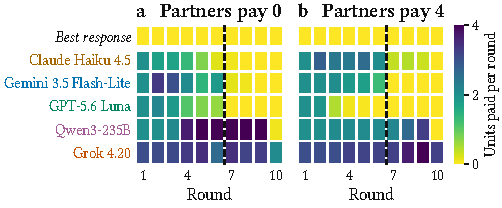
\includegraphics[width=\columnwidth]{figures/fig_scripted.pdf}
\Description{Two heatmaps with one row per model and one column per round, beside five
partners that always pay nothing and beside five that always pay four. Darker cells mean
larger payments. The top row, the best response, is light everywhere. GPT Luna's row turns
light within a few rounds and Gemini Flash-Lite and Claude Haiku turn light at a dashed line
after round six, while Qwen and Grok stay dark until round nine.}
\caption{One model beside five scripted partners, pooled over five risk levels (50 games per
row). A cell is the mean payment in one round; the top row is the best response, 0 in every
round. The dashed rule follows round 6, after which the outcome is settled in most games.}
\label{fig:scripted}
\end{figure}

\begin{table}[t]
\caption{Units a model pays per game before and after the outcome is settled, beside five
partners who always pay 0 or always pay 4 (50 games per entry). Given these partners, every
unit paid is wasted; units paid after settlement are wasted even for an agent that does not
know its partners are scripted.}
\label{tab:settled}
\small
% Generated by paper/AAMAS/analysis/scripted.py. Do not edit by hand.
\begin{tabular}{@{}lrrrr@{}}
\toprule
 & \multicolumn{2}{c}{Always 0} & \multicolumn{2}{c}{Always 4} \\
\cmidrule(lr){2-3}\cmidrule(l){4-5}
Model & Before & After & Before & After \\
\midrule
Claude Haiku 4.5 & 7.7 & 0.1 & 14.2 & 1.1 \\
Gemini 3.5 Flash-Lite & 13.6 & 0.2 & 10.9 & 0.0 \\
GPT-5.6 Luna & 8.5 & 0.0 & 4.5 & 0.0 \\
Qwen3-235B & 17.8 & 12.1 & 12.3 & 8.1 \\
Grok 4.20 & 19.6 & 11.1 & 16.7 & 16.2 \\
\bottomrule
\end{tabular}

\end{table}

\paragraph{Responses to partners take simple forms.}
The models respond to their partners, but not the way a best responder would
(Figure~\ref{fig:scripted}, Table~\ref{tab:settled}). Gemini Flash-Lite and Claude Haiku pay their usual
rate and then stop once the history shows that the outcome is settled. GPT Luna pays little even
before that point, above all beside partners who always pay 4, which is close to a best
response while it learns who its partners are. Qwen raises its payment to 4 beside partners
who pay nothing. Qwen and Grok keep paying large amounts after the outcome is settled, which
no belief about the partners can justify. Qwen's last-round rule also costs its partners:
beside five fair-share partners it pays 2 for nine rounds and then 0, and the table misses the
target in \ScrQwenFairMiss{} of 50 games, each time by exactly \ScrQwenFairShort{} units.
Gemini Flash-Lite in the same seat reaches the target in \ScrFlashFairReach{} of 50.

%% =====================================================================================
%% 6 Mixed tables, and 7 selection among agents.
%% Numbers: tables/num_mixed.tex (analysis/mixed.py), tables/num_advantage.tex
%% (analysis/advantage.py), tables/num_selection.tex (analysis/selection.py).
%% Figures: fig_advantage.pdf, fig_mixed.pdf, fig_selection.pdf.
%% Design fact, do not "fix": seat blocks are contiguous and fixed within each
%% (pair, seats) cell; the order of the two blocks alternates across cells, so every
%% model holds every seat equally often only when cells are pooled.
%% The within-table ranking follows from Proposition 2; present it as known selection
%% theory made concrete, and put the empirical weight on who pays least in company and on
%% what selection costs the group.
%% =====================================================================================
\section{Defaults in mixed groups}
\label{sec:groups}

Self-play and scripted partners cannot show what happens when agents with different defaults
share a table. We seat every pair of models together, with one to five seats for the first
model, at $p\in\{0.1,0.5,0.9\}$ and ten games per cell, for \MixGames{} games. The seats of
each model form one block whose position is fixed within a cell and alternates across cells,
so every model holds every seat equally often overall.

\begin{figure}[t]
\centering
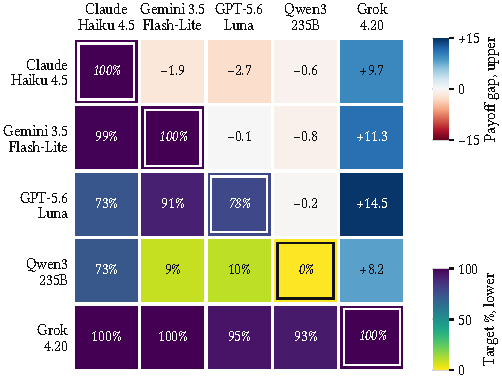
\includegraphics[width=\columnwidth]{figures/fig_advantage.pdf}
\Description{One five-by-five matrix over pairs of models, split along the diagonal. Cells
above the diagonal give the payoff of the row model's seats minus that of the column model's
seats at the same table; the Grok column is blue, meaning every other model earns more than
Grok, and the other cells are pale, meaning small differences. Cells on and below the diagonal
give the share of games that reach the target; the cells that pair Qwen with Gemini
Flash-Lite or GPT Luna are nearly white, and the Grok row is dark.}
\caption{Two models at one table, 150 games per pair, pooled over seat splits and risk. Above
the diagonal: expected payoff of the row model's seats minus the column model's, in the same
games. On and below it: share of games reaching the target; boxed cells are self-play (60
games).}
\label{fig:advantage}
\end{figure}

At a shared table every model earns more than Grok, by up to \AdvMaxAbs{} units per seat,
while the payoff gaps among the other four are small (Figure~\ref{fig:advantage}, above the
diagonal). This
follows from Proposition~\ref{prop:table}: Grok pays the most, and at one table the larger
payer earns less. Group success depends on the pair (Figure~\ref{fig:advantage}, below the
diagonal). Tables
that include Grok almost always reach the target, while tables that mix Qwen with Gemini Flash-Lite
or GPT Luna rarely do; \AdvPairLowReachName{} succeed in only \AdvPairLowReachPct\% of their
games.

\begin{figure}[t]
\centering
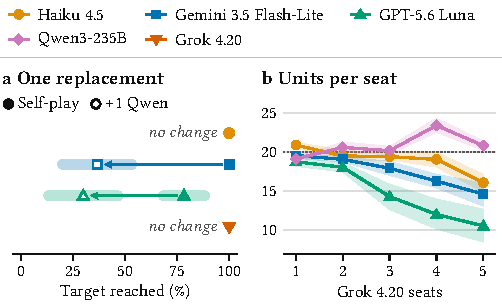
\includegraphics[width=\columnwidth]{figures/fig_mixed.pdf}
\Description{Two dot charts with one row per model, where an arrow runs from a filled marker
to an open marker. Left: the share of games reaching the target, alone and with one seat
replaced by Qwen; the arrows for Gemini Flash-Lite and GPT Luna run far to the left, while
Claude Haiku and Grok stay at full success. Right: what a seat pays beside one Grok seat and
beside five; the arrows for GPT Luna, Gemini Flash-Lite and Claude Haiku run left, below the
fair share, while Qwen moves slightly right.}
\caption{Two models at one table, pooled over $p$. Arrows run from the filled marker to the
open one, which carries a 95\% interval. (a)~Target reached by six seats of one model (60
games) and by five seats plus one Qwen seat (30). (b)~What a seat pays beside one and five Grok
seats (30 games each; dots: two to four); dotted: the fair share.}
\label{fig:mixed}
\end{figure}

\paragraph{An exact fair share has no slack.}
One partner that stops paying in the last round is enough to break a table of exact
fair-share players (Figure~\ref{fig:mixed}a). When the pool stands at 108 before round 10,
Qwen pays nothing in \MixQwenPotZeroPct\% of its decisions, against \MixFlashPotZeroPct\% for
Gemini Flash-Lite. Five Gemini Flash-Lite seats with one Qwen seat therefore succeed in only
\MixFlashQwenReach{} of 30 games, although Gemini Flash-Lite alone never misses, and five GPT
Luna seats with one Qwen seat succeed in \MixLunaQwenReach{} of 30, against
\MixLunaAloneReach\% alone. Claude Haiku and Grok tables, which pay more than needed, absorb
the same partner (\MixHaikuQwenReach{} of 30 for Claude Haiku). In \MixQwenPivotalFix\% of the
\MixMissWithQwen{} missed tables with a Qwen seat, turning its last-round zeros into 2s would
have reached the target. Slack also works the other way: one Grok seat lets five Qwen seats
reach the target in \MixGrokRescuesQwen{} of 30 games, and Grok pays for the rescue. Since
Qwen's last-round rule depends on the wording, this measures what one late dropout does to a
group, whichever model plays that role.

\paragraph{Generous partners are under-matched.}
Agents pay less, not more, when generous partners fill most of the table
(Figure~\ref{fig:mixed}b). Next to five Grok seats, GPT Luna pays \MixLunaBesideFiveGrok{} units
per seat, against \MixLunaBesideOthers{} next to other partners, and Gemini Flash-Lite and
Claude Haiku pay \MixFlashBesideFiveGrok{} and \MixHaikuBesideFiveGrok{}. As with scripted
partners, Gemini Flash-Lite and Claude Haiku stop once the pool reaches the target, while GPT
Luna pays less from the start, so the generous partner carries the group. Qwen pays slightly
more beside Grok. These responses fit watching the pool, which our design does not separate
from tracking who paid.

\section{Which agent wins under selection}
\label{sec:selection}

Systems that host many agents keep some and drop others: an operator picks the agent that
earned most, or users copy the one that did well. The key question is whom an agent is
compared with, and we show that the answer decides which of our five models such a process
favours. Following empirical game-theoretic
analysis~\cite{wellman2006methods,tuyls2018generalised}, each model is a strategy. We write
$\pi_A(k)$ for the mean expected payoff of an $A$ seat at a table with $k$ seats of $A$ and
$6-k$ seats of another model $B$, estimated from the mixed tables for $1\le k\le5$ and from
self-play for $k=6$.

\paragraph{Selection process.}
A population of $N$ agents holds $i$ agents of type $A$ and $N-i$ of type $B$, and tables of
six are drawn at random. The fitness of each type is its payoff averaged over the tables it
can land in, as given by
\begin{align}
f_A(i) &= \textstyle\sum_{k=1}^{6} \mathcal{H}(k-1;\,N-1,\,i-1)\;\pi_A(k), \label{eq:fitness}\\
f_B(i) &= \textstyle\sum_{k=0}^{5} \mathcal{H}(k;\,N-1,\,i)\;\pi_B(6-k), \nonumber
\end{align}
where $\mathcal{H}(k;\,N-1,\,m)$ is the hypergeometric chance that $k$ of the five other seats
come from the $m$ other agents of type $A$. An agent copies a random other agent with
probability $1/(1+e^{-\beta\Delta f})$, where $\Delta f$ is their fitness gap and $\beta$ is
the selection intensity, set to 1 per payoff unit. $\alpha$-Rank~\cite{omidshafiei2019alpha}
assumes that a new model enters rarely, so the population is almost always made of one model.
It computes the chance that a single newcomer takes over, for every pair of models, and turns
these chances into a Markov chain over the five one-model populations. The share of time the
chain spends on each model is the weight selection gives it, its \emph{stationary mass}. The
population size sets whom an agent is compared with. With $N=6$ the whole population is one
table, so an agent is compared only with its tablemates. With $N=30$, fitness is averaged over
random tables, so an agent is compared mostly with agents who sat elsewhere.

\paragraph{Scoring against tablemates rewards the smallest payer.}
Within one table, Proposition~\ref{prop:table} fixes the ranking before any data are seen:
the seat that pays less earns more. What the data add is who pays least in company, which is
Qwen, and what this selection costs. It gives Qwen the largest weight at every risk level
(Figure~\ref{fig:selection}, top row). The selected population then reaches the target in only
\SelWithinReachMid\% of games at $p=0.5$ and \SelWithinReachHigh\% at $p=0.9$, against
\SelUniformReachMid\% and \SelUniformReachHigh\% for a model picked at random. With stronger
selection ($\beta=\SelBetaExtra$) the success rate falls to \SelStrongWithinReachMid\% and
\SelStrongWithinReachHigh\%. This is the known result that selection on payoff relative to a
small group favours whoever does better than its neighbours, even at a cost to the
group~\cite{schaffer1988evolutionarily}, now shown with language-model agents.

\begin{figure}[t]
\centering
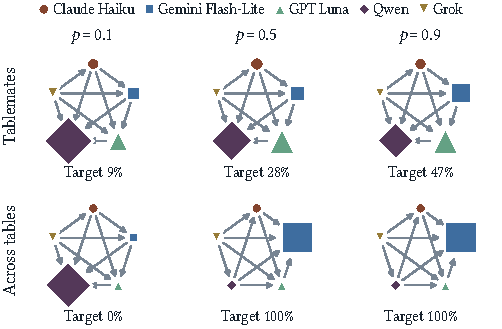
\includegraphics[width=\columnwidth]{figures/fig_selection.pdf}
\Description{Six small graphs in two rows and three columns, one column per catastrophe
probability 0.1, 0.5 and 0.9. Each graph has five nodes, one per model, arranged in a
pentagon, with arrows between every pair. Top row, comparison with tablemates: the Qwen node
is the largest at every risk level and the target rates printed below are low. Bottom row,
comparison across tables: the Qwen node is largest at 0.1, and the Gemini Flash-Lite node is
largest at 0.5 and 0.9, where the target rate is 100 percent.}
\caption{Which model selection favours ($\alpha$-Rank, $\beta=1$). A node is a one-model
population, larger when it gets more stationary mass; an arrow points to the model whose
newcomer takes over more easily. Top: $N=6$, so agents are compared with their tablemates.
Bottom: $N=30$, so mostly with agents at other tables. Under each graph: the self-play target
rate, weighted by mass.}
\label{fig:selection}
\end{figure}

\paragraph{Scoring across tables keeps the fair-share player.}
When agents are compared with agents at other tables, what matters is how well a model's own
tables do. At $p=0.5$ and $0.9$ selection then favours Gemini Flash-Lite
(Figure~\ref{fig:selection}, bottom row), whose population reaches the target in \SelAcrossReachHigh\%
of games at $p=0.9$ and earns the optimum, \SelAcrossPayHigh{} units per seat. It wins because
it is rigid: a newcomer that pays less pushes its table below the target, and one that pays
more loses money. At $p=0.1$ both rules favour \SelAcrossWinnerLow{}, which still earns far
less than the optimum, since every model pays at low risk. The winners do not change with
stronger selection, with populations of \SelNExtra{} agents, or when self-play payoffs use
only the risk grid, and each stays on top in at least \SelBootMinPct\% of bootstrap samples.
Under weak selection ($\beta=\SelWeakBeta$) no model gets more than \SelWeakWithinMaxMass{} of
the weight within a table, so the cost of tablemate scoring needs selection that is at least
moderately strong. The same
agents, scored in two reasonable ways, lead to opposite outcomes for the group, in line with
theory on selection between groups~\cite{traulsen2006evolution}, and tablemate scoring is one
simple route to the selfish outcomes that imitation produced for model-written
strategies~\cite{willis2026evaluating}.

%% =====================================================================================
%% 8 Discussion, threats to validity, limitations, ethics.
%% Do not promise reproducibility of model text: replaying the same cell with the same
%% seed gives different play. Promise the design (prompts, configurations, seeds, code).
%% The "must"/unstated-goal threat is no longer untested: the neutral-wording and
%% goal-stated arms answer it (Section 4). Keep the remaining threats honest.
%% =====================================================================================
\section{Discussion}
\label{sec:discussion}

No model grades its payments by the size of the risk under the base prompt. Four models pay
a default of their own, close to the fair share or well above it, and still pay at $p=0$,
where paying helps no one, so generosity alone cannot explain their play. GPT Luna stops at
$p=0$ but pays the same share at every positive risk. The default does not come from
normative wording. It appears when the goal is left unstated, and stating the goal removes
most payment at zero risk without making most models weigh the risk. All five adjust to
partners only in simple ways, mostly by stopping once the outcome is settled.

\paragraph{Possible causes.}
Our data record choices, not reasoning, so we offer hypotheses. First, the equal split may be
a focal point, a choice everyone expects everyone else to make; models rebuild it without the
hint, and a 50/50 split can likewise reflect a focal point rather than a
preference~\cite{dodivers2025uncovering}. Second, a question may call up computation and a
move request a default, which fits reports that models can hold a correct belief or plan and
act against it~\cite{fan2024can,schmied2026llms}. Third, post-training may favour doing one's
share when nothing says otherwise, which fits the finding that models are more cooperative
than people~\cite{mei2024turing} and our finding that naming the goal removes most payment at
zero risk. Stronger reasoning is not an obvious fix, since reasoning models free-ride more in
public goods games~\cite{guzmanpiedrahita2025corrupted}.

\paragraph{Consequences for design.}
\emph{State the agent's goal.} An agent that is told only the rules falls back on a default,
and one sentence naming its goal removed the payment at zero risk that neutral wording left in
place. Evaluations should report what the agent was told to want.
\emph{Test against the optimum, not the success rate.} A group can reach its target in every
game and still waste most of its money, so a study needs $\mathrm{opt}(p)$, a condition where
paying is dominated, such as $p=0$, and a check for payment after the outcome is settled.
\emph{Test in mixed populations.} Self-play hides how defaults interact: an exact fair-share
default is optimal among copies of itself and fragile next to one late dropout, while a
generous default absorbs that partner and pays for others. \emph{Choose the selection signal
with care.} Any leaderboard, market or imitation process that scores an agent against its
tablemates favours whoever pays least, by Proposition~\ref{prop:table}, and in our games this
lowered group success, while scoring across independent groups favoured the agent whose
groups succeed. Each test needs only the game rules, a few scripted policies or a second
model, and each caught a failure that self-play success rates did not show.

\paragraph{Threats to validity.}
The goal sentence is itself an instruction, and we test one phrasing of it, at three risk
levels, in self-play only. Two other features of the setup may push models toward paying, and
neither is tested here. The decision prompt asks for a final line with the move, so models
may deliberate less when deciding than when answering a question. And the game is well
known, so the fair share may be recalled rather than derived; the neutral wording removes the
game's name, but the rules still describe it. The same prompts were used for every model, so
these features cannot explain why the models differ, but they may raise the common level of
payment.

\paragraph{Limitations.}
We test five low-cost models, one per provider, in English and in one game; more capable
models may respond to risk~\cite{anon-if}, so our claims are about this tier. Cells hold ten
games, which limits power for the noisiest model, Grok. Our rewordings test wording, not
every prompt design. The welfare losses assume risk-neutral players; the two tests where
paying is dominated do not. The scripted partners, mixed tables and selection analysis use the
base prompt only; mixed tables hold two models with fixed seat blocks within a cell, and
$\alpha$-Rank assumes rare entry. For four models the self-play grid was collected separately;
a rerun of the same prompt matches it (Table~\ref{tab:robust}). Model text is not
reproducible, so we release prompts, configurations, seeds and code, and promise
reproducibility of the design rather than of the transcripts.

\paragraph{Ethics.}
The study involves no human subjects and no personal data. Its findings describe failure
modes of deployed systems, and we report them so that designers can test for them before
agents are trusted with shared resources.


\clearpage
\bibliographystyle{ACM-Reference-Format}
\bibliography{refs}

\end{document}
